\documentclass{exam}
\usepackage{../../mypackages}
\usepackage{../../macros}
\usepackage{scrextend}
\usepackage{paralist}
\usepackage{enumitem}
%\usepackage{blindtext}

\renewcommand{\arraystretch}{1.5} % Augmente l'espacement vertical entre les lignes du tableau
\newcolumntype{C}{>{\centering\arraybackslash}m{2cm}}

\SetLabelAlign{myright}{\hss\llap{$#1$}}
\newlist{where}{description}{1}
\setlist[where]{labelwidth=2cm,labelsep=1em,
                        leftmargin=!,align=myright,font=\normalfont}

\setlength{\parindent}{0pt}

\title{Devoir sur table N°1}
\author{N. Bancel}
\date{2 Décembre 2024}

\begin{document}


\textbf{Collège Lycée Suger}
\hfill
\textbf{Physique-Chimie} \\

\textbf{Année 2024-2025}
\hfill
\textbf{3ème Cambridge International} \par

{\let\newpage\relax\maketitle}
%\maketitle


  \begin{center}
    \textbf{\textcolor{blue}{Durée du devoir : 2 heures}} \par
    \vspace{1em}
    \textbf{\textcolor{red}{La calculatrice EST autorisée. Total des points : 20.5 points}} \par
    \vspace{1em}
  \end{center}
  
  \begin{tcolorbox}[colback=gray!10!white, colframe=gray, title=Note importante]
    Toutes les réponses doivent être justifiées : une réponse sans justification est considérée comme fausse. \par
    \vspace{1em}
    Il est permis d'admettre le résultat de certaines questions pour ne pas rester bloqué, en prenant soin d'indiquer sur la copie les résultats admis. \par
    \vspace{1em}
    Des points bonus seront attribués si les résultats sont écrits en notation scientifique (type $a \times 10^n$), ou si la rédaction est particulièrement soignée. \par
    \vspace{1em}
    Barème des points (les exercices peuvent être traités dans le désordre)
    \begin{itemize}
      \item Exercice 1 : 2.5 points
      \item Exercice 2 : 5 points
      \item Exercice 3 : 4 points
      \item Exercice 4 : 3 points
      \item Exercice 5 : 6 points
  \end{itemize}
  \end{tcolorbox}

\section*{Exercice 1 - Les soldats (2.5 points)}

Le prix du plomb ayant fortement augmenté ces dernières années, des escrocs remplacent le plomb utilisé pour fabriquer des figurines par de l'acier (composé majoritairement de fer, moins cher). Les soldats ci-contre sont-ils en plomb ou en acier ?


\begin{tcolorbox}[colback=gray!10!white, colframe=green!75!black, title=\textcolor{black}{Document 1 - Caractéristiques d'un lot de \textbf{25} soldats de plomb}]
  \begin{itemize}
    \item Masse totale : \textbf{1.4 kg}
    \item Volume de métal utilisé par soldat : \textbf{5 $cm^3$}
  \end{itemize}
\end{tcolorbox}

\begin{figure}[H]
  \centering
  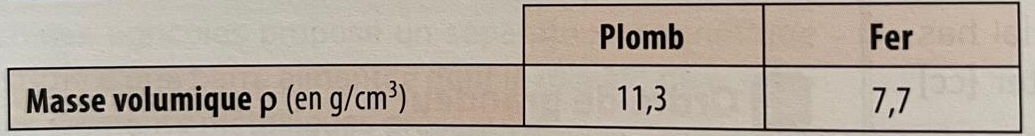
\includegraphics[width=0.8\linewidth]{img/dst_1_01.png}
  \caption{Document 2 - Masse volumique du plomb et du fer}
\end{figure} 


\begin{questions}
  \question[1] Estimer en grammes la masse d'un soldat de plomb.
  \question[1] Calculer la masse volumique du matériau composant les soldats.
  \question[0.5] En déduire le matériau utilisé pour fabriquer les soldats.
\end{questions}

\section*{Exercice 2 - L'atome - 5 points}

\begin{questions}
  \question[2] Compléter la figure ci-dessous. Il est obligatoire de donner une justification de la méthode en amont (pas besoin de la ré expliquer à chaque fois). Aucun point ne sera attribué si aucune justification n'est apportée.

\begin{table}[H]
  \centering
  \begin{tabularx}{\textwidth}{|X|C|C|C|C|}
  %\begin{tabularx}{\textwidth}{|X|c|c|c|c|}
    \hline
    \textbf{Symbole de l’atome} & \textbf{C} & \textbf{Ne} & \textbf{Al} & \textbf{Zn} \\
    \hline
    \textbf{Nom de l’atome} & carbone & néon & aluminium & zinc \\
    \hline
    \textbf{Nombre d’électrons} & 6 & 10 & ... & 30 \\
    \hline
    \textbf{Nombre de nucléons} & 12 & 20 & 27 & ... \\
    \hline
    \textbf{Nombre de protons} & ... & ... & 13 & ... \\
    \hline
    \textbf{Nombre de neutrons} & ... & ... & ... & 35 \\
    \hline
  \end{tabularx}
\end{table}

\question[1]  Expliquer pourquoi l'atome est électriquement neutre

\question[2] (Extrait du brevet 2023) L'eau de mer contient, au moins en petites quantités, de nombreux éléments chimiques. Parmi ceux-ci, le sodium est présent sous forme d’ion dans le chlorure de sodium. On
donne ci-dessous un extrait de la classification périodique des éléments chimiques qui les
regroupe par ordre croissant de numéro atomique (nombre de protons dans le noyau de
l’élément considéré).

\begin{figure}[H]
  \centering
  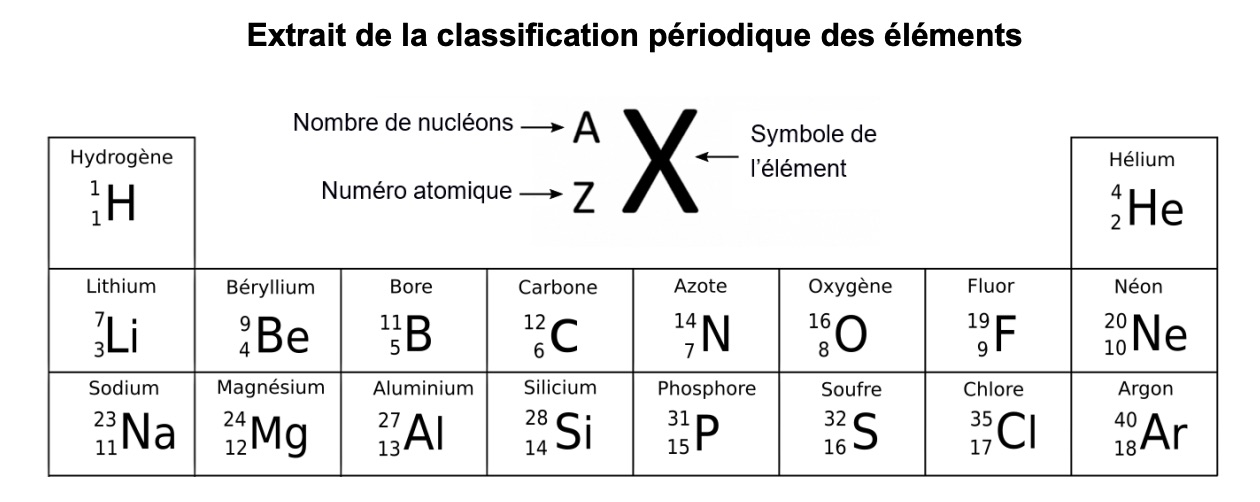
\includegraphics[width=0.8\linewidth]{img/dst_1_02.jpg}
  \caption{Tableau périodique}
\end{figure} 

\begin{parts}
  \part[0.5] Donner le symbole de l'élément sodium 
  \part[0.5] Donner le nombre de protons contenus dans le noyau d’un atome de sodium.
  \part[1] Indiquer le nombre de neutrons contenus dans le noyau d’un atome de sodium.
Expliquer la démarche
\end{parts}

\end{questions}

\section*{Exercice 3 - Les incendies - 4 points}

Lors d’un incendie de forêt, les arbres subissent une réaction de combustion. Le bois, assimilé à de
la cellulose de formule chimique simplifiée \ce{C6H10O5}, réagit avec le dioxygène et produit du dioxyde
de carbone et de l’eau à l’état gazeux. L’équation de la réaction est :

\begin{center}
  \ce{C6H10O5 + 6 O2 -> 6 CO2 + 5 H2O}
\end{center}

\begin{questions}
  \question[1.5] L'équation de réaction ci-dessus est-elle équilibrée ? Justifier.
  \question[1] Lister, \textbf{en Français (et non pas avec la formule scientifique / chimique)}, les réactifs et les produits de cette équation
  \question[1] On fait réagir du \ce{C6H10O5} et de l'\ce{O2} comme dans la réaction ci-dessus. La masse totale des réactifs est de \SI{52}{kg}. Quelle est la masse de la combinaison de \ce{CO2} et de \ce{H2O} produite ? Justifier. 
  \question[0.5] (Bonus) A partir de l'équation de réaction, justifier que les incendies produisent des gaz à effet de serre.
\end{questions}


\section*{Exercice 4 - Déduction de formules (3 points)}

\begin{tcolorbox}[colback=gray!10!white, colframe=gray, title=Document 1 - La vitesse]
  Contexte : La vitesse d'un objet peut se calculer en mesurant en distance, et en déterminant le temps qu'il a fallu à cet objet pour parcourir cette distance. Sa formule s'écrit
  \[
  v = \frac{d}{t}
  \]
  où 

  \begin{addmargin}[4em]{1em}
    \begin{compactitem}
        \item [v]: représente la vitesse de l'objet
        \item [d]: représente la distance parcourue
        \item [t]: représente le temps écoulé pour que l'objet parcourt la distance
    \end{compactitem}
    \end{addmargin}
  \end{tcolorbox}

\begin{tcolorbox}[colback=gray!10!white, colframe=gray, title=Document 1 - L'énergie cinétique]
  Contexte : Lorsque vous voyez une voiture en mouvement, son énergie (cinétique) dépend de sa vitesse et de sa masse. Cette énergie joue un rôle important lors des accidents de voiture ou dans la conception des freins. Sa formule est 
  \[
  E_c = \frac{1}{2} \times m \times v^2
  \]
  où 
  \begin{addmargin}[4em]{1em}
  \begin{compactitem}
    \item [$E_c$]: représente l'énergie cinétique de l'objet
    \item [m]: représente la masse de l'objet 
    \item [v]: représente la vitesse de l'objet
\end{compactitem}
\end{addmargin}

  
\end{tcolorbox}

\begin{questions}
  \question[1] Si dans un problème, je connais la valeur de la vitesse d'un véhicule, et je sais combien de temps il a roulé, comment puis-je déduire la distance qu'il a parcourue ?
  \question[1] Si dans un problème, je connais la valeur de la vitesse d'un véhicule, et je sais quelle distance il a parcouru, comment puis-je déduire le temps / la durée pendant laquelle il a roulé ?
  \question[1] Si dans un problème, je connais la valeur de l'énergie cinétique et je connais la valeur de la vitesse, quelle formule me permet de déterminer la masse de l'objet ?
\end{questions}

\section*{Exercice 5 - Conversions et autres petits exercices (6 points)}

\begin{questions}
  \question[1] Equilibrer l'équation de réaction suivante : \ce{C + O2 -> CO}. Justifier.
  \question[1] Equilibrer l'équation de réaction suivante : \ce{N2 + H2 -> NH3}. Justifier.
  \question[1] Effectuer la conversion suivante : \( 0,0024 \, \mathrm{km} \) à convertir en \textbf{cm}. Justifier.
  \question[1] Effectuer la conversion suivante : \( 2,5 \, \mathrm{g/cL} \) à convertir en  \textbf{kg/L}. Justifier.
  \question[2] A partir des données ci-dessous, calculer la valeur de $\frac{m_{nucléon}}{m_{electron}}$ (où $m_{nucléon}$ représente la masse d'un nucléon et où $m_{electron}$ représente la masse d'un électron). En déduire que la masse d'un atome est pratiquement égale à la masse de son noyau.

  \begin{center}
    \begin{tabular}{SS}
      \toprule
      {Constituant} & {Masse (en \si{kg})} \\
      \midrule
      {Electron} & {\(9.1 \times 10^{-31}\)} \\
      {Nucléon (Proton et Neutron)} & {\(1.7 \times 10^{-27}\)} \\
      \bottomrule
    \end{tabular}
  \end{center}
\end{questions}


\end{document}
